
	\documentclass{article}
	\usepackage{amsmath,amssymb}
	\usepackage[inline]{enumitem}
	\usepackage{blindtext}
	\usepackage{booktabs}
	\usepackage{graphicx}
	\usepackage{xcolor}
	\usepackage[vmargin = 1.5in, top = 1in, bottom = 1.2in, letterpaper]{geometry}
	\usepackage{listings}
	\usepackage{courier}
	\usepackage{multicol}
	\usepackage{multirow}
	\usepackage{bm}
	\usepackage{subcaption}
	\lstset{
	basicstyle = \small\tt,
	keywordstyle = \tt\color{blue},
	commentstyle = \it\color[cmyk]{1,0,1,0},
	stringstyle = \tt\color[RGB]{128,0,0},
	%frame = single,
	backgroundcolor = \color[RGB]{245,245,244},
	breaklines,
	extendedchars = false,
	xleftmargin = 2em,
	xrightmargin = 2em,
	aboveskip = 1em,
	tabsize = 4,
	showspaces = false
	}
	\begin{document}
	
	% \newfontfamily\courier{Courier New}

	
	\title{STAT 520 Homework 4}
	\author{Yifan Zhu}
	\maketitle
	
	\begin{enumerate}[leftmargin = 0 em, label = 4.\arabic*., font = \bfseries]
	\item 
	\begin{enumerate}
		\item
		Random variable in this problem is the nitrogren concentration of well $i$, denoted $Y_i$. And the covariate is indicator variable $x_{ik}$ for $i = 1, \cdots, n$ and $k = 1,2,3$, where
		\[x_{ik} = \begin{cases}
			1 & \textrm{well $i$ is in county $k$}\\
			0 & \textrm{otherwise}
		\end{cases}\]


		\item 
		For $Y_i$ from the same county, it follows a Gamma distribution with mean $\mu_k$, where $\mu_k = \alpha/\beta_k$ and $Y_i$'s are independent. The parameters used in the model are $\theta_1, \theta_2, \theta_3$, which represent the true mean for each county, and
		\[\mu_i = \sum_{k=1}^3 x_{ik} \theta_k, \quad i = 1,2,\ldots, n\]
		where $\mu_i = E(Y_i)$.

		\item 
		The estimation of $\theta_k$ and the standard errors are shown in Table \ref{1par}
		\begin{table}[!htb]
		\caption{Estimation of parameter and standard error}
		\label{1par}
		\centering
			\begin{tabular}{lll}
			\toprule
				Parameter & Estimation & SE\\
				\midrule
				$\theta_1$ & 4.249 & 0.4937\\
				$\theta_2$ & 4.577 & 0.5326\\
				$\theta_3$ & 4.192 & 0.4877\\
				\bottomrule
			\end{tabular}
		\end{table}

		\item 
		We construct the simutanuous confidence interval using the Bonferroni method by constructing the 98.3\% confidence interval. Then we have Table \ref{simu_ci}
		\begin{table}[!htb]
		\caption{95\% simutanuous confidence interval}
		\label{simu_ci}
		\centering
			\begin{tabular}{lll}
			\toprule
				Parameter & Simutaneous Interval \\
				\midrule
				$\theta_1$ & (3.192, 5.294) \\
				$\theta_2$ & (3.444, 5.711) \\
				$\theta_3$ & (3.152, 5.229) \\
				\bottomrule
			\end{tabular}
		\end{table}

	 Figure \ref{simu_ci_g} shows the overlapping of three confidence intervals. 
	 \begin{figure}[!htb]
	 	\centering
	 	\includegraphics[width = 0.75\textwidth]{simu_ci.eps}
	 	\caption{95 \% Simutaneous Intervals}
	 	\label{simu_ci_g}
	 \end{figure}

	From Figure \ref{simu_ci_g} we find that there is a lot overlapping between these three confidence intervals, thus we can conclude that there is no sufficient evidence that the true mean of nitrogreon concentrations are different.

	\item 
	From the previous analysis, we conclude that $\theta_1 = \theta_2 = \theta_3 = \theta$. So we fit a glm with
	\[\mu_i = \theta. i = 1,\ldots, n\]
	We get $\hat{\theta} = 4.337, \hat{\phi} = 3.031$. Thus the Gamma distribution would have parameter $\alpha = 3.031, \beta = 0.6988$. The density plot is shown in Figure \ref{gamma}
	\begin{figure}[!htb]
		\centering
		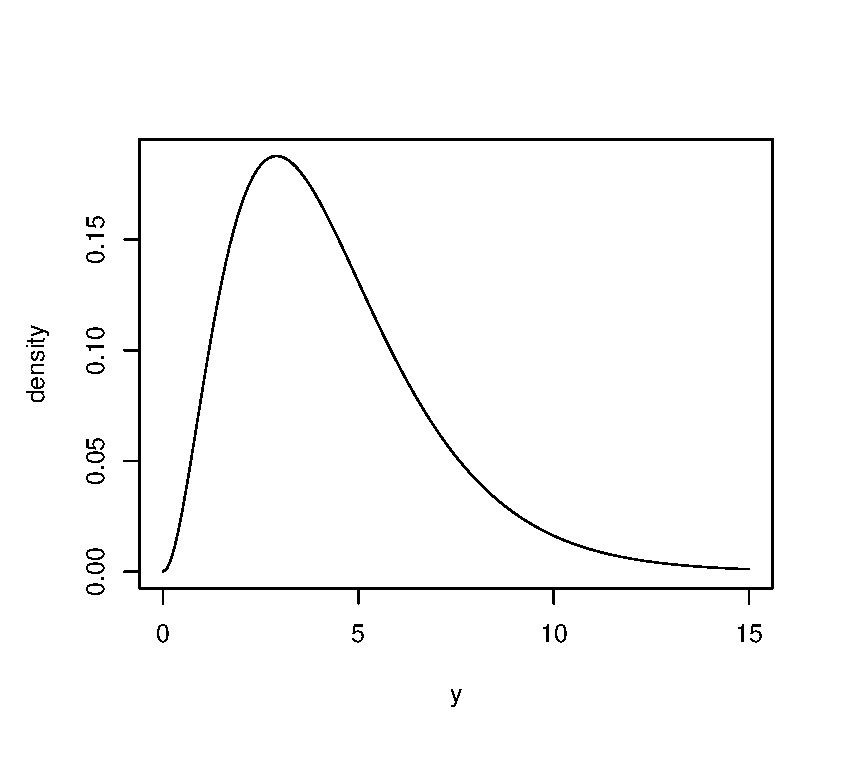
\includegraphics[width = 0.75\textwidth]{gamma.eps}
		\caption{Density of the estimated common gamma distribution}
		\label{gamma}
	\end{figure}

	And with those estimated parameters, we have $P(Y \leq 3) = 0.3421$ and $P(Y \geq 10) = 0.0310$.

	\end{enumerate}
	\newpage
	\item 
	\begin{enumerate}
		\item 
		The random variables are $Y_{ik}$, where $i = 1,\ldots, n_k$ and $k = 1,2,3$. $n_k$ is the number if wells sampled in the $k$-th county, and $Y_{ik}$ is the nitrate concentration of the $i$-th well in county $k$.

		\item 
		In order to conduct a likelihood analysis, we fit two models. One reduced model with 3 different gamma distributions with different parameters $(\alpha_k, \beta_k)$ and a reduced model with only one gamma distribution with parameter $(\alpha, \beta)$. 

		Let $f(y| \alpha, \beta)$ be the pdf of gamma distribution with parameters $\alpha$ and $\beta$, then the log likelihood for the full model is
		\[\ell_F  = \sum_{k=1}^3 \sum_{i = 1}^{n_k} \log (f(y_{ik}| \alpha_k, \beta_k))\]

		And for the reduced model, log likelihood is 
		\[\ell_R = \sum_{k=1}^3 \sum_{i = 1}^{n_k} \log (f(y_{ik})| \alpha , \beta)\]

		\newpage

		\item 
		The MLE's for the parameters in the full and reduced model are shown in Table \ref{est2}.
		\begin{table}[!htb]
			\centering
			\caption{Estimation and Standard Error for parameters}
			\label{est2}
			\begin{tabular}{lll}
			\toprule
			Parameter & Estimation &  SE\\ 
			\midrule
			$\alpha_1$ & 1.778 & 0.4635 \\
			$\beta_1$ & 0.419 & 0.1260 \\
			$\alpha_2$ & 3.578 & 1.0193\\
			$\beta_2$ & 0.821 & 0.2382 \\
			$\alpha_3$ & 6.603 & 1.822 \\
			$\beta_3$ & 1.575 & 0.4517\\
			$\alpha$ & 3.010 & 0.4669\\
			$\beta$ & 0.694 & 0.1171\\
			\bottomrule 
			\end{tabular}
				
		\end{table}


		\item 
		When we plug in MLE into these two models, we can get $\ell_F$ and $\ell_R$ mentioned in (b). Then we have the value of $\Lambda$ which follows asymptotically a Chi-square distribution with 2 degrees of freedom. And
		\[\Lambda = -2 (\ell_R - \ell_F) = 12.212\]
		That gave us a p-value $p = 0.01584$. Thus we reject the reduced model and conclude that the nitrate concentrations in wells for different counties follows different distributions.

		In order to compare with the analysis we did in 4.1, we calculated the estimation for each $\hat{\mu}_k = \frac{\hat{\alpha}_k}{\hat{\beta}_k}$ and the their standard error using Delta method. And then we produced the 95\% simultaneous confidence intervals. The results are shown in Table
		\begin{table}[!htb]
		   	\centering
		   	\caption{Estimation, standard error and 95\% simultaneous interval for $\mu_k$}
		   	\label{simu2}
		   	\begin{tabular}{llll}
		   	\toprule
		   		Parameter & Estimation & SE & 95\% simultaneous interval\\ 
		   		\midrule
		   		$\mu_1$ & 4.243 & 0.6364 & (2.8892, 5.5968)\\
		   		$\mu_2$ & 4.577 & 0.4722 & (3.5725, 5.5815)\\
		   		$\mu_3$ & 4.192 & 0.3262 & (3.4981, 4.8859)\\
		   		\bottomrule
		   	\end{tabular}
		   \end{table}  

		Figure \ref{simu2_g} shows the overlapping of these 3 simultaneous intervals, from which we can see there is still a lot a overlapping although our conclusion is these three distributions are different. 
     \begin{figure}[!htb]
	 	\centering
	 	\includegraphics[width = 0.75\textwidth]{simu2.eps}
	 	\caption{95 \% Simutaneous Intervals}
	 	\label{simu2_g}
	 \end{figure}

	 \item 
	 From the previous analysis, our conclusion is that there is sufficient evidence that the nitrate concentration in wells from different counties are different. The probabilities are given in Table 
	 \ref{prob}. Figure \ref{den2} shows the pdf's of three gamma distributions.

	 		\begin{table}[!htb]
		   	\centering
		   	\caption{Probabilities}
		   	\label{prob}
		   	\begin{tabular}{lll}
		   	\toprule
		   		County & $P(Y < 3)$ & $P(Y>10)$ \\ 
		   		\midrule
		   		$1$ & 0.4292 & 0.0587 \\
		   		$2$ & 0.2786 & 0.0286 \\
		   		$3$ & 0.2480 & 0.0032 \\
		   		\bottomrule
		   	\end{tabular}
		   \end{table} 

\begin{figure}[!htb]
	 	\centering
	 	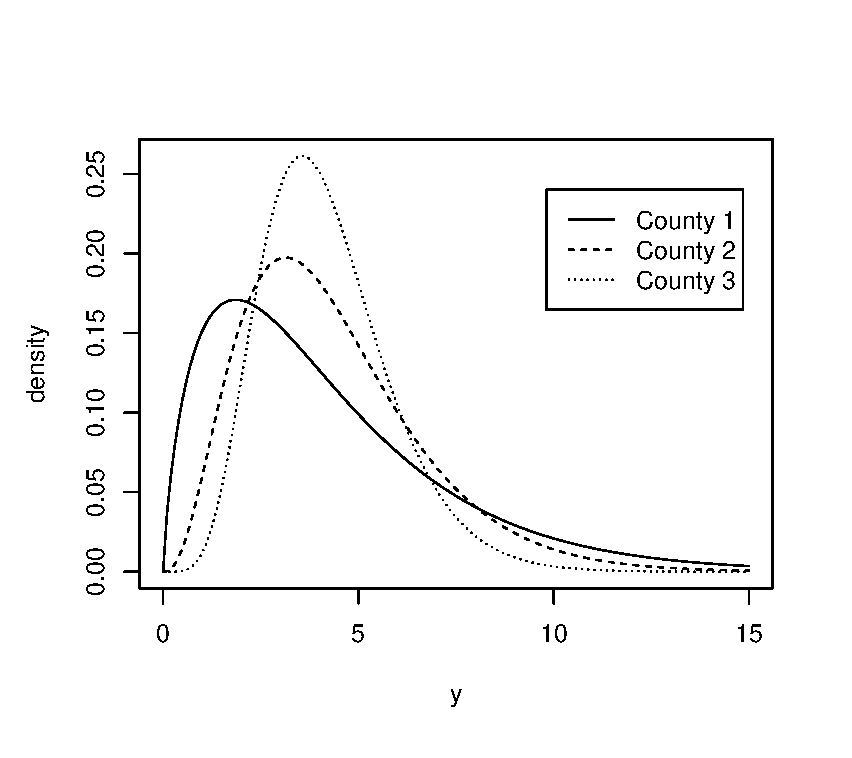
\includegraphics[width = 0.7\textwidth]{dens2.eps}
	 	\caption{Density of estimated gamma distributions for three counties}
	 	\label{den2}
	 \end{figure}

	\end{enumerate}

\newpage
	\item In these two analyses, we get two different conclusions for different test. For the first one using simultaneous intervals, we conclude that there is no sufficient evidence that the means of nitrate concentration in wells of 3 counties are different. For the second analysis, we conclude that there is sufficient evidence that the distributions of nitrate concentration for 3 counties are different. The different conclusions are resulted from different hypothesis and different tests conducted. In the second analysis, when we construct the simultaneous intervals like the first analysis, we get a similar conclusion about the mean of nitrate concentration.

	

 	\end{enumerate}


	
	
	
	\end{document}